\documentclass[11pt,a4paper]{article}

\usepackage[spanish]{babel}
\usepackage[math,light]{iwona}
\usepackage[utf8]{inputenc}
\usepackage{amsmath, amsthm}
\usepackage{amsfonts, amssymb, latexsym}
\usepackage{enumerate}
\usepackage[usenames, dvipsnames]{color}
\usepackage{graphics,graphicx, float} %para incluir imágenes y colocarlas
\usepackage{colortbl}
\usepackage{graphicx}
\usepackage{wrapfig}
\usepackage[top=4cm]{geometry}
\usepackage{cite}
\usepackage[official]{eurosym}
\usepackage{cancel}
\usepackage{subfigure}
\usepackage{minted}

\theoremstyle{plain}
\newtheorem{exe}{Ejercicio} % reset theorem numbering for each chapter

\theoremstyle{definition}
\newtheorem{sol}{Solución}

\usepackage[bookmarks=true,
            bookmarksnumbered=false, % true means bookmarks in
                                     % left window are numbered
            bookmarksopen=false,     % true means only level 1
                                     % are displayed.
            colorlinks=true,
            linkcolor=webblue,
            citecolor=red]{hyperref}
\definecolor{webgreen}{rgb}{0, 0.5, 0} % less intense green
\definecolor{webblue}{rgb}{0, 0, 0.5}  % less intense blue
\definecolor{webred}{rgb}{0.5, 0, 0}   % less intense red

\setlength{\parindent}{0pt}
\setlength{\parskip}{1ex plus 0.5ex minus 0.2ex}

\newcommand{\HRule}{\rule{\linewidth}{0.5mm}}

\title{\Huge{Visión por Computador} \\ Práctica 1}
\author{Marta Gómez Macías}

\begin{document}

\maketitle

\tableofcontents

\section{Opción desarrollada}

Antes de empezar la práctica, aclarar que he escogido la \textbf{opción 1}.

\section{Convolución de una imagen con una máscara}
\subsection{Cálculo del vector máscara}

A continuación se muestran las funciones encargadas de calcular la máscara:

\begin{minted}[frame=lines, label={Cálculo de la máscara}]{python}
# función gaussiana para la máscara
kernel = lambda x, sigma: exp(-0.5 * ((x*x)/(sigma*sigma)))

# Función para calcular la máscara/kernel
def my_getGaussianKernel(sigma):
    # El tamaño de la máscara depende de sigma. Aplicando la estadística báisca, 
    # llegamos a que lo óptimo es tomar 3sigma por cada lado. Por lo que el 
    # tamaño de la máscara será 6sigma + 1
    mascara = np.arange(-floor(3*sigma),floor(3*sigma + 1))
    # aplicamos la gaussiana a la máscara
    mascara = np.array([kernel(m, sigma) for m in mascara])
    # y la devolvemos normalizada
    return np.divide(mascara, np.sum(mascara))
\end{minted}

La función \texttt{kernel} es una función auxiliar de la función \texttt{my\_getGaussianKernel}. Ésta última está inspirada en la función de \textit{OpenCV} \texttt{getGaussianKernel} y su función es devolver la máscara que más tarde se usará para filtrar la imagen.

A diferencia de la función \texttt{getGaussianKernel} de \textit{OpenCV}, \texttt{my\_getGaussianKernel} calcula el tamaño de la máscara en función de $\sigma$:

\begin{displaymath}
 M\acute{a}scara = \bigg[\lfloor-3\sigma\rfloor,\lfloor3\sigma\rfloor\bigg]
\end{displaymath}

por ejemplo, si $\sigma = 1$, la máscara tendría tamaño 7 y abarcaría el intervalo $[-3,3]$. El redondeo es necesario ya que $\sigma$ es un número real, pero la máscara sólo puede abarcar números enteros.

Una vez que la función obtiene el tamaño de la máscara, pasa a calcular cada valor de la misma. Para ello, se usa la siguiente expresión matemática definida en la función \texttt{kernel}:

\begin{displaymath}
 f(x) = exp \Bigg(-0.5 \cdot \frac{x^2}{\sigma^2} \Bigg)
 \end{displaymath}

Y, por último, la función normaliza los valores obtenidos para que la suma total de la máscara sea 1.

\subsection{Convolución 2D con un filtro Gaussiano}
\subsubsection{Convolución 1D de dos vectores}

En el caso de la gaussiana, la correlación y la convolución obtienen el mismo resultado. Aprovechando esta propiedad, se ha implementado sólo la correlación. Esta función se utiliza más adelante, en la función que hace la convolución 2D con una gaussiana (\hyperref[sec:conv2D]{Sección \ref*{sec:conv2D}}).

\begin{minted}[frame=lines, label={Correlación de dos vectores 1D}]{python}
# Función para aplicar el kernel a un trocito de imagen
apply_kernel = lambda original, kernel: np.sum(original * kernel)
\end{minted}

Gracias a la librería \texttt{numpy} de python y a las funciones $\lambda$ podemos implementar esta función en una sola línea.

\subsubsection{Relleno de los extemos de la imagen usando distintos criterios de borde}

Para poder elegir distintos tipos de borde, se ha implementado una función ``interfaz'' que aplica el tipo de borde que escojamos.

\begin{minted}[frame=lines, label={Añadir borde a una imagen}]{python}
# Función para añadir borde a una imagen
def my_copyMakeBorder(src, space, borderType):
    return {
        'black':black_border(src, space),
        'replicate':replicate_border(src,space),
        'reflect':reflect_border(src,space),
        'reflect_101':reflect_101_border(src,space),
        'wrap':wrap_border(src,space)
    }.get(borderType)
\end{minted}

Se han implementado los mismos tipos de bordes que implementa \textit{OpenCV}:

\begin{enumerate}[$\qquad\bullet$]
\item \textbf{Constante}: aplica un borde negro a la imagen. En la \hyperref[black]{Figura \ref*{black}} vemos el resultado de aplicar este tipo de borde a una imagen. Para ello, aumenta el tamaño de cada fila y cada columna en $k$ (siendo $k$ el tamaño de la máscara menos 1) y añade en el centro la imagen. Esta función es bastante importante, porque es sobre la que están basadas el resto de funciones de borde.

\begin{minted}[frame=lines, label={Borde negro}]{python}
# Función para darle a la imagen un borde negro 
# BORDER_CONSTANT: iiiiii | abcdefgh | iiiiiii
def black_border(src, space):
    # creamos una imagen negra
    if len(src.shape) == 3:
        img_borde = np.zeros((src.shape[0]+space*2, src.shape[1]+space*2,3), \
            np.uint8)
    else:
        img_borde = np.zeros((src.shape[0]+space*2, src.shape[1]+space*2), \
            np.uint8)
    dims = img_borde.shape
    # copiamos en el centro la imagen original
    img_borde[space:dims[0]-space, space:dims[1]-space] = src
    return img_borde
\end{minted}

\begin{figure}[!h]
    \centering
    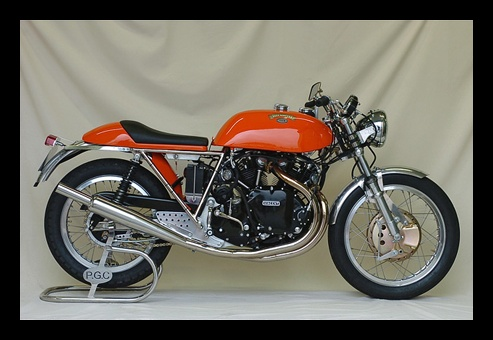
\includegraphics[width=0.7\textwidth]{borde_negro}
    \caption{Resultado de aplicar la función \texttt{black\_border} sobre una imagen}
    \label{black}
\end{figure}

\item \textbf{Replicado}: copia el último pixel de cada fila/columna. En la \hyperref[replicate]{Figura \ref*{replicate}} vemos el resultado de aplicar este tipo de borde a una imagen. Para ello, aplica un borde negro a la imagen, usando la función \texttt{black\_border} y una vez hecho eso, rellena dicho borde negro con dos bucles \texttt{for}: uno para copiar el primer y último píxel por filas y otro para hacerlo por columnas.

\begin{minted}[frame=lines, label={Borde replicado}]{python}
# Función para darle a la imagen un borde 
# BORDER_REPLICATE: aaaaaa | abcdefgh | hhhhhhh
def replicate_border(src, space):
    # le añadimos un borde negro a la imagen
    img_borde = black_border(src,space)
    # cambiamos ese borde negro por una copia del último píxel. Primero por filas
    dims = src.shape
    for fila in range(dims[0]):
        img_borde[space+fila,0:space] = src[fila,0]
        img_borde[space+fila,dims[1]+space:dims[1]+2*space] = src[fila,dims[1]-1]
    # después, por columnas
    for columna in range(dims[1]):
        img_borde[0:space,columna+space] = src[0,columna]
        img_borde[dims[0]+space:dims[0]+2*space,space+columna] = \
        src[dims[0]-1,columna]
    return img_borde
\end{minted}

\begin{figure}[!h]
    \centering
    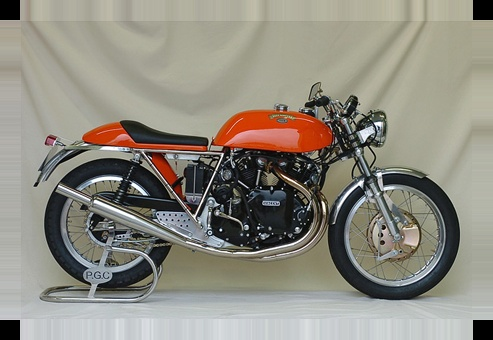
\includegraphics[width=0.7\textwidth]{borde_replicado}
    \caption{Resultado de aplicar la función \texttt{replicate\_border} sobre una imagen}
    \label{replicate}
\end{figure}

\item El resto de bordes que implementa \textit{OpenCV} (reflejado, reflejado 101 y envuelto) se implementan de la misma forma que éste último y por eso no han sido incluidos en esta memoria.

\end{enumerate}

% \item \textbf{Reflejado}: refleja en el borde los últimos píxeles de la imagen. En la \hyperref[reflect]{Figura \ref*{reflect}} vemos el resultado de aplicar este tipo de borde a una imagen. 

% \begin{minted}[frame=lines, label={Borde reflejado}]{python}
% # Función para reflejar la imagen
% # BORDER_REFLECT: fedcba | abcdefgh | hgfedcb
% def reflect_border(src,space):
%     # le añadimos un borde negro a la imagen
%     img_borde = black_border(src,space)
%     # cambiamos ese borde negro por copias de los space primeros píxeles 
%     # de la imagen
%     dims = src.shape
%     for fila in range(dims[0]):
%         to_copy_left = np.array(src[fila, 0:space])
%         img_borde[space + fila, 0:space] = to_copy_left[::-1]
%         to_copy_right = src[fila, dims[1]-space-1:dims[1] - 1]
%         img_borde[space + fila, dims[1] + space:dims[1] + 2 * space] = \
%         to_copy_right[::-1]

%     for columna in range(dims[1]):
%         to_copy_left = np.array(src[0:space, columna])
%         img_borde[0:space, columna + space] = to_copy_left[::-1]
%         to_copy_right = np.array(src[dims[0]-space-1:dims[0] - 1, columna])
%         img_borde[dims[0] + space:dims[0] + 2 * space, space + columna] = \
%         to_copy_right[::-1]
%     return img_borde
% \end{minted}

% \begin{figure}[!h]
%     \centering
%     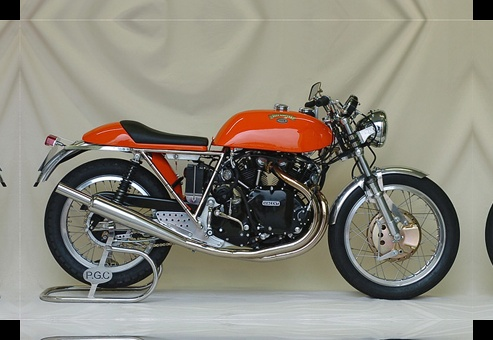
\includegraphics[width=0.7\textwidth]{borde_reflejado}
%     \caption{Resultado de aplicar la función \texttt{reflect\_border} sobre una imagen}
%     \label{reflect}
% \end{figure}

% \item \textbf{Reflejado 101}: igual que la anterior, pero empieza a reflejar desde el penúltimo píxel. En la \hyperref[reflect101]{Figura \ref*{reflect101}} vemos el resultado de aplicar este tipo de borde a una imagen.

% \begin{minted}[frame=lines, label={Borde reflejado 101}]{python}
% # Función para reflejar la imagen
% # BORDER_REFLECT_101: gfedcb | abcdefgh| gfedcba
% def reflect_101_border(src,space):
%     # le añadimos un borde negro a la imagen
%     img_borde = black_border(src,space)
%     # cambiamos ese borde por los space+1 primeros píxeles de 
%     # la imagen, sin contar el primero de todos
%     dims = src.shape
%     for fila in range(dims[0]):
%         to_copy_left = np.array(src[fila, 1:space+1])
%         img_borde[space + fila, 0:space] = to_copy_left[::-1]
%         to_copy_right = src[fila, dims[1]-space-2:dims[1] - 2]
%         img_borde[space + fila, dims[1] + space:dims[1] + 2 * space] = \
%         to_copy_right[::-1]

%     for columna in range(dims[1]):
%         to_copy_left = np.array(src[1:space+1, columna])
%         img_borde[0:space, columna + space] = to_copy_left[::-1]
%         to_copy_right = np.array(src[dims[0]-space-2:dims[0] - 2, columna])
%         img_borde[dims[0] + space:dims[0] + 2 * space, space + columna] = \
%         to_copy_right[::-1]
%     return img_borde
% \end{minted}

% \begin{figure}[!h]
%     \centering
%     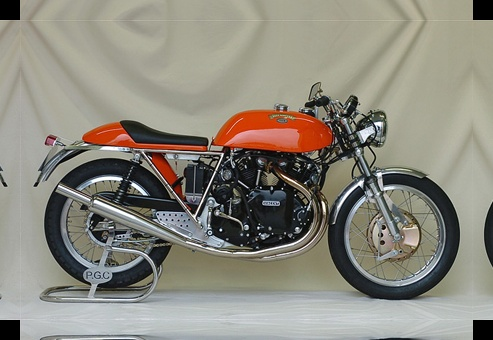
\includegraphics[width=0.7\textwidth]{borde_reflejado101}
%     \caption{Resultado de aplicar la función \texttt{reflect\_101\_border} sobre una imagen}
%     \label{reflect101}
% \end{figure}

% \item \textbf{Envuelto}: refleja los últimos píxeles del lado contrario. En la \hyperref[wrap]{Figura \ref*{wrap}} vemos el resultado de aplicar este tipo de borde a una imagen.

% \begin{minted}[frame=lines, label={Borde envuelto}]{python}
% # Función que continua el borde que la imagen deja por el lado contrario
% # BORDER_WRAP: cdefgh | abcdefgh | abcdefg
% def wrap_border(src,space):
%     # le añadimos un borde negro a la imagen
%     img_borde = black_border(src, space)
%     # cambiamos ese borde negro por copias de los space primeros 
%     # píxeles de la imagen
%     dims = src.shape
%     for fila in range(dims[0]):
%         to_copy_left = np.array(src[fila, 0:space])
%         to_copy_right = src[fila, dims[1] - space - 1:dims[1] - 1]
%         img_borde[space + fila, 0:space] = to_copy_right[::-1]
%         img_borde[space + fila, dims[1] + space:dims[1] + 2 * space] = \
%         to_copy_left[::-1]

%     for columna in range(dims[1]):
%         to_copy_left = np.array(src[0:space, columna])
%         to_copy_right = np.array(src[dims[0] - space - 1:dims[0] - 1, columna])
%         img_borde[0:space, columna + space] = to_copy_right[::-1]
%         img_borde[dims[0] + space:dims[0] + 2 * space, space + columna] = \
%         to_copy_left[::-1]
%     return img_borde
% \end{minted}

% \begin{figure}[!h]
%     \centering
%     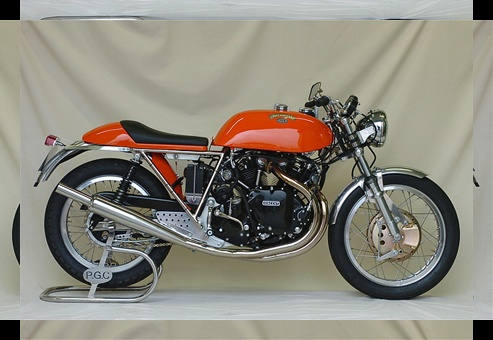
\includegraphics[width=0.7\textwidth]{borde_wrap}
%     \caption{Resultado de aplicar la función \texttt{wrap\_border} sobre una imagen}
%     \label{wrap}
% \end{figure}
% \end{enumerate}

Como se aprecia, no se aplica el borde a los píxeles de las esquinas. Este detalle se ha obviado debido a que las esquinas no influyen en el cálculo de la convolución de la imagen.


\subsubsection{Aplicar las funciones anteriores a una imagen separando canales si fuese necesario}\label{sec:conv2D}

Se han desarrollado dos funciones: \texttt{my\_filter2D} y \texttt{my\_filter2D\_onechannel}. La primera función sirve como interfaz de la segunda.

\begin{minted}[frame=lines, label={Convolución 2D}]{python}
# Función para aplicar la máscara 1D a una imagen con más de un canal
def my_filter2D(src, kernel, borderType):
    # en primer lugar comprobamos si la imagen es en color o en blanco y negro
    if len(src.shape) == 3:
        # si es en color, debemos separar sus canales
        canales = cv2.split(src)
        # y aplicar sobre cada uno de ellos el filtro
        for i in range(len(canales)):
            canales[i] = my_filter2D_onechannel(src=canales[i], kernel=kernel,\
                borderType=borderType)
        # una vez hecho esto, los volvemos a juntar con merge
        img = cv2.merge(canales)
    else:
        # si solo tiene un canal, aplicamos directamente el filtro
        img = my_filter2D_onechannel(src=src, kernel=kernel, \
            borderType=borderType)
    return img
\end{minted}

La función \texttt{my\_filter2D} comprueba en primer lugar si la imagen es en color o en blanco y negro. Para ello, comprueba el tamaño del atributo \texttt{shape} de la imagen de entrada. A continuación, si la imagen resulta ser en color, separa sus canales usando la función \texttt{split} de \textit{OpenCV} y aplica el filtro gaussiano sobre cada canal. Por último, una vez aplicado el filtro sobre cada canal, se vuelven a juntar en una sola imagen usando la función \texttt{merge} de \textit{OpenCV}. Si la imagen resulta ser en blanco y negro, se le aplica directamente el filtro.

\begin{minted}[frame=lines,label={Convolución 2D en blanco y negro}]{python}
# Función para aplicar la máscara 1D a un canal de la imagen
def my_filter2D_onechannel(src, kernel, borderType):
    mitad_mascara = floor(kernel.size/2)
    # En primer lugar, añadimos bordes a la imagen
    img_bordes = my_copyMakeBorder(src=src, space=mitad_mascara, borderType=borderType)
    img_aux = np.ones(img_bordes.shape, np.uint8)*255
    # Después, aplicamos el kernel a cada trocito
    for j in range(mitad_mascara, img_bordes.shape[0]-mitad_mascara):
        for i in range(mitad_mascara,img_bordes.shape[1]-mitad_mascara):
            img_aux[j,i] = apply_kernel(img_bordes[j,i-mitad_mascara:\
                i+1+mitad_mascara], kernel)
    img_bordes = img_aux.copy(order='F')
    img_aux = np.ones(img_bordes.shape, np.uint8)*255
    # Después, aplicamos el kernel a cada trocito
    for j in range(mitad_mascara, img_bordes.shape[1]-mitad_mascara):
        for i in range(mitad_mascara,img_bordes.shape[0]-mitad_mascara):
            img_aux[i,j] = apply_kernel(img_bordes[i-mitad_mascara:\
                i+1+mitad_mascara,j], kernel)
    img_bordes = img_aux.copy(order='F')
    # Devolvemos la imagen con el filtro aplicado
    return img_bordes[mitad_mascara:-mitad_mascara, mitad_mascara:-mitad_mascara]
\end{minted}

La función \texttt{my\_filter2D\_onechannel} es la que aplica el filtro sobre un único canal. Para ello, calcula en primer lugar la mitad del tamaño de la máscara para saber el espacio que tiene que dejar en cada borde la imagen. Tras esto, aplica un borde (especificado por parámetro) a la imagen. Usando la imagen con bordes, empezamos a aplicar el filtro a la imagen usando la función \texttt{apply\_kernel}, \textbf{primero por filas y después por columnas}. Me ha parecido mejor hacerlo así en vez de hacerlo en una función a parte y trasponer la imagen por cuestiones de eficiencia. Es importante destarcar que el filtro debe aplicarse sobre una imagen copia auxiliar para no arrastrar el filtro a lo largo de toda la imagen.

En \hyperref[convolucion]{Figura \ref*{convolucion}} se muesta cómo funciona la función con $\sigma = 1$ y se compara con el resultado que obtiene \textit{OpenCV} con el mismo parámetro. En comparación con \textit{OpenCV}, me da la sensación de que \textit{OpenCV} sólo aplica la máscara en una dimensión, ya que el desenfoque obtenido con \textit{OpenCV} da la sensación de movimiento vertical. En cambio, el resultado obtenido con la función \texttt{my\_filter2D} sí que da la sensación de un desenfoque ``uniforme''.

\begin{figure}[!h]
    \centering
    \mbox {
    \subfigure[Resultado obtenido con la función \texttt{getGaussianKernel} de \textit{OpenCV}, usando como parámetros $k_{size} = 7$ y $\sigma=1$]{
    \label{opencv1}
    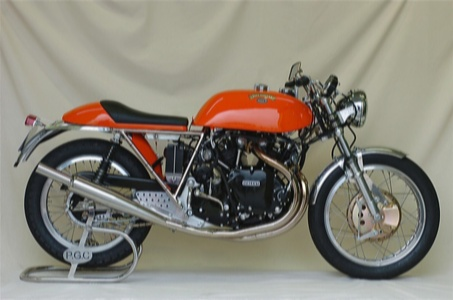
\includegraphics[width=0.5\textwidth]{opencv_sigma2}
    }
    \qquad
    \subfigure[Resultado obtenido con la función \texttt{my\_getGaussianKernel}, usando como parámetro $\sigma=1$] {
    \label{propio1}
    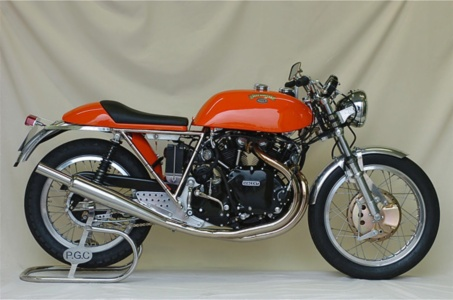
\includegraphics[width=0.5\textwidth]{propio_sigma2}
    }
    }
    \mbox{
    \subfigure[Resultado obtenido con la función \texttt{getGaussianKernel} de \textit{OpenCV}, usando como parámetros $k_{size} = 19$ y $\sigma=3$]{
    \label{opencv1}
    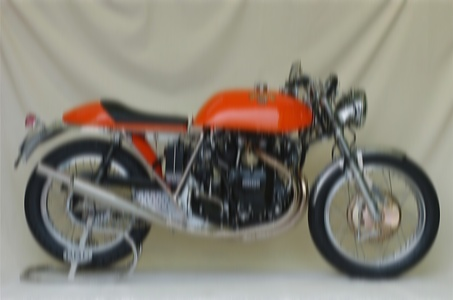
\includegraphics[width=0.5\textwidth]{opencv_sigma3}
    }
    \qquad
    \subfigure[Resultado obtenido con la función \texttt{my\_getGaussianKernel}, usando como parámetro $\sigma=3$] {
    \label{propio1}
    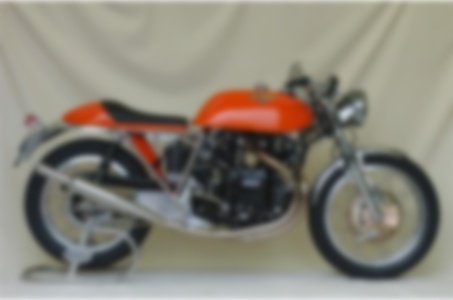
\includegraphics[width=0.5\textwidth]{propio_sigma3}
    }
    }
    \caption{Comparación entre el filtro gaussiano de \textit{OpenCV} y el desarrollado para la práctica.}
    \label{convolucion}
\end{figure}

\section{Imágenes híbridas}

Las imágenes híbridas son un efecto óptico en el cual engañamos al ojo haciéndole creer que ve una cosa distinta si mira la imagen de cerca o la mira de lejos. Para ello, mezclamos las \textbf{frecuencias altas} de una imagen con las \textbf{frecuencias bajas} de otra. 

A parte de la función de convolución (\texttt{my\_filter2D}) desarrollada, he hecho dos más: una llamada \texttt{hybrid} que toma como parámetros dos imágenes y los distintos $\sigma$ que aplicar a cada una y otra llamada \texttt{make\_collage} que sirve para hacer un collage a partir de varias imágenes. Ésta última no ha sido incluida en el guión debido a que no tiene ningún aspecto de implementación que destacar.

Para hacer una imagen híbrida, he aplicado a ambas imágenes una máscara de convolución para obtener así las frecuencias bajas de cada una. Para obtener las frecuencias altas, he restado a la imagen original la imagen con las frecuencias bajas. Por último, para obtener la imagen híbrida, he sumado las frecuencias bajas de una imagen con las frecuencias altas de la otra imagen. 

He añadido a la función un parámetro para dejar que el usuario decida si quiere el resultado en forma de collage o no. En el caso de que el usuario quiera el resultado en forma de collage, obtendrá como resultado un collage con las tres imágenes: la imagen con frecuencias bajas, la imagen con frecuencias altas y la híbrida de ambas.

\begin{minted}[frame=lines, label={Funciones para hacer imágenes híbridas}]{python}
def hybrid(img_alta,img_baja,space=210,sigma_alta=1.5,sigma_baja=4.5,collage=True):
    # obtenemos las máscara respectivas para cada imagen
    my_mascara_alto = my_getGaussianKernel(sigma=sigma_alta)
    my_mascara_bajo = my_getGaussianKernel(sigma=sigma_baja)
    # leemos las dos imágenes que vamos a mezclar
    img = cv2.imread(img_alta, cv2.IMREAD_UNCHANGED)
    img2 = cv2.imread(img_baja, cv2.IMREAD_UNCHANGED)
    # para quedarnos con las frecuencias altas de la imagen, restamos las 
    # frecuencias bajas que obtenemos con el filtro gaussiano a la 
    # imagen original
    paso_alto = img - my_filter2D(src=img, kernel=my_mascara_alto, \
        borderType='replicate')
    paso_bajo = my_filter2D(src=img2, kernel=my_mascara_bajo, \
        borderType='replicate')
    # para obtener la imagen híbrida, sumamos las dos imágenes.
    if collage:
        return make_collage([paso_bajo,paso_alto,paso_alto+paso_bajo],\
            ["Low","High","Both"],space)
    else:
        return paso_alto+paso_bajo
\end{minted}

\begin{figure}[!h]
    \centering
    \subfigure[Resultado tras mezclar las frecuencias bajas de \textit{Marilyn Monroe} con las frecuencias altas de \textit{Albert Einstein}]{
    \label{einsrilyn}
    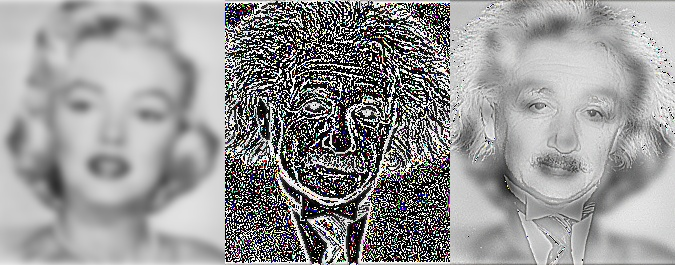
\includegraphics[width=0.75\textwidth]{einsrilyn}
    }
    \subfigure[Resultado tras mezclar las frecuencias bajas de un pájaro con las frecuencias altas de un avión] {
    \label{birdplane}
    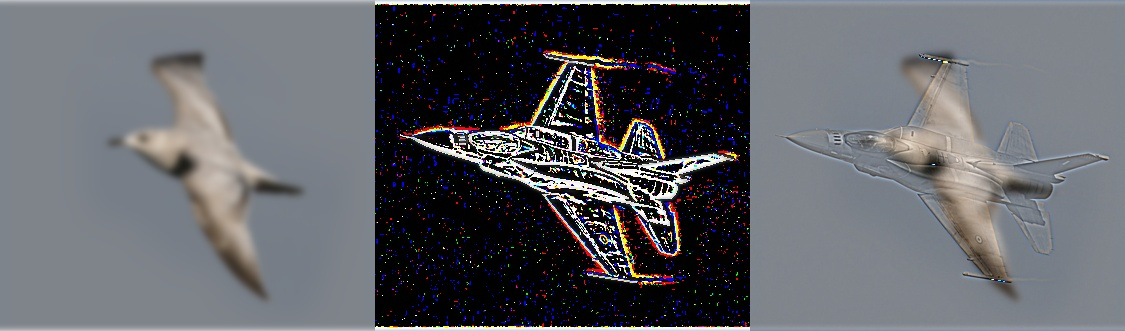
\includegraphics[width=0.75\textwidth]{birdplane}
    }
    \subfigure[Resultado tras mezclar las frecuencias bajas de un perro con las frecuencias altas de un gato]{
    \label{catdog}
    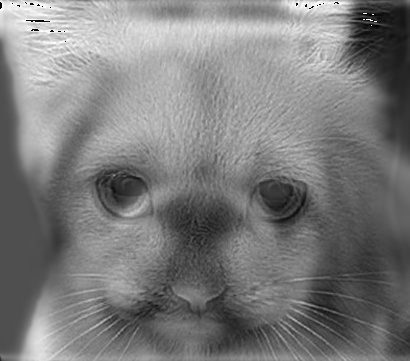
\includegraphics[width=0.5\textwidth]{catdog}
    }
    \caption{Ejemplos de imágenes híbridas}
    \label{hybrid}
\end{figure}

En la \hyperref[hybrid]{Figura \ref*{hybrid}} tenemos algunos ejemplos de imágenes híbridas hechas con esta función.

\section{Pirámides Gaussianas}

Las \textbf{pirámides gaussianas} son un collage en el que se representa una misma imagen en distintas escalas: 1/1, 1/2, 1/4...

Para hacer la pirámide gaussiana de una imagen, he desarrollado dos funciones: \texttt{resize} para escalar una una imagen con un parámetro $scale$, de forma $\frac{1}{scale}$ y \texttt{piramide\_gaussiana} para crear la pirámide.

En la función \textbf{piramide\_gaussiana}, creo un canvas con tamaño:

\begin{displaymath}
size_{canvas} = \bigg [ ancho_{canvas} + \frac{ancho_{canvas}}{2}, alto_{canvas} \bigg ]
\end{displaymath}

Una vez creado el canvas, se coloca la imagen original en la parte izquierda y, se hace un bucle para colocar el resto de imágenes escaladas a la derecha. Se colocan las siguientes escalas: 1/2, 1/4, 1/8 y 1/16.

Es importante destacar que para escalar una imagen hay que seguir dos pasos: primero aplicar un filtro gaussiano para eliminar ruido y, después, redimensionar la imagen. Si no se hace esto, la imagen escalada tendrá demasiado ruido.

\begin{minted}[frame=lines, label={Pirámides Gaussianas}]{python}
# Función para redimensionar una imagen 1/scala de su tamaño.
def resize(img, scale):
    # Para hacer un buen redimensionado. Debemos primero aplicar un filtro 
    # gaussiano a la imagen y después quedarnos con las filas/columnas %scale. 
    # Por ejemplo si scale=2, sólo nos quedaríamos con las pares.
    img_blur = my_filter2D(src=img, kernel=my_getGaussianKernel(scale/2),\
        borderType='replicate')
    # una vez desenfocada la imagen, creamos una nueva imagen para 
    # guardarla y nos quedamos con las filas/columnas %scale
    img_little = img_blur[range(0,img_blur.shape[0],scale)]
    img_little = img_little[:,range(0,img_blur.shape[1],scale)]

    return img_little

# Función para hacer un collage tipo pirámide gaussiana
def piramide_gaussiana(img, scale=5):
    # el tamaño del canvas debe ser: 
    # ancho_img_original + 0.5*ancho_img_original x altura_img_original
    dims = img.shape
    if len(dims) == 3:
        piramide = np.ones((dims[0],dims[1]+floor(dims[1] * 0.5),3),\
            np.uint8)*255
    else:
        piramide = np.ones((dims[0], dims[1] + floor(dims[1] * 0.5)),\
            np.uint8) * 255

    # colocamos la primera imagen en tamaño original
    piramide[0:dims[0],0:dims[1]] = img
    # calculamos el lugar donde poner la segunda
    start_height = 0
    end_height = ceil(dims[0]/2)
    start_width = dims[1]   # este lugar será igual para todas las imágenes
    start_width -= 1
    little = img
    for i in range(2,scale+1):
        # calculamos la i-esima imagen
        little = resize(img=little, scale=2)
        # guardamos sus medidas
        dims = little.shape
        # la colocamos en el sitio calculado
        piramide[start_height:end_height,start_width:start_width+dims[1]] = little
        # calculamos dónde colocar la siguiente imagen
        start_height = end_height
        end_height = ceil(dims[0]/2) + start_height

    return piramide
\end{minted}

\begin{figure}[!h]
    \centering
    \mbox{
    \subfigure[Pirámide gaussiana de la imagen híbrida hecha entre \textit{Albert Einstein} y \textit{Marilyn Monroe}]{
    \label{einsrilyn}
    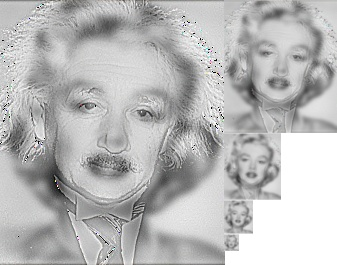
\includegraphics[width=0.5\textwidth]{piramide_einsrilyn}
    }
    \qquad
    \subfigure[Pirámide gaussiana de la imagen híbrida hecha entre un perro y un gato]{
    \label{catdog}
    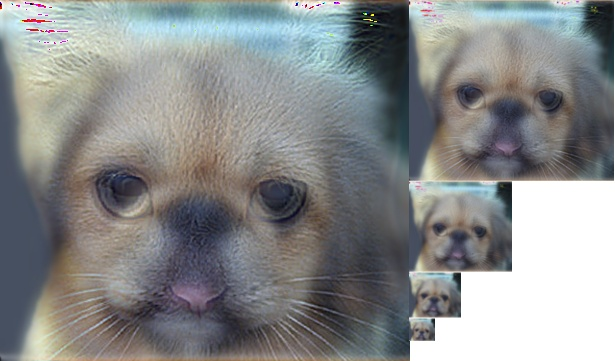
\includegraphics[width=0.5\textwidth]{piramide_catdog}
    }
    }
    \mbox{
    \subfigure[Pirámide gaussiana de la imagen híbrida hecha entre un avión y un pájaro]{
    \label{einsrilyn}
    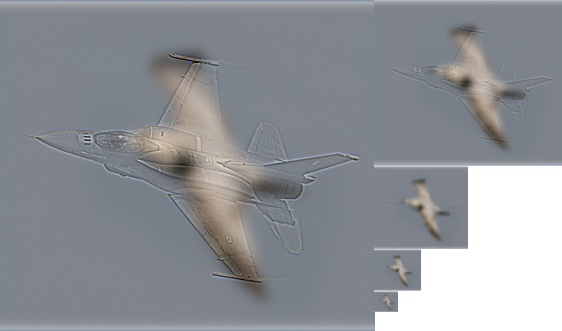
\includegraphics[width=0.5\textwidth]{piramide_birdplane}
    }
    \qquad
    \subfigure[Pirámide gaussiana de la imagen híbrida hecha entre un pez y un submarino]{
    \label{catdog}
    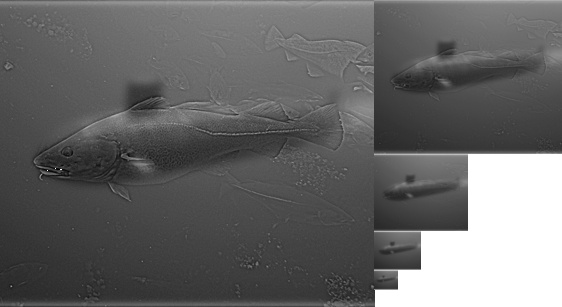
\includegraphics[width=0.5\textwidth]{piramide_fishsub}
    }
    }
    \caption{Ejemplos de pirámides gaussianas}
    \label{piramide}
\end{figure}

Por ejemplo, en las imágenes de la \hyperref[piramide]{Figura \ref*{piramide}}. De ver un gato pasamos a ver un perro y de ver a \textit{Albert Einstein} pasamos a ver a \textit{Marilyn Monroe}. Esto se debe a que cuando escalamos una imagen perdemos detalles de la misma, tanto por eliminar filas y columnas como por aplicar un filtro gaussiano cada vez que escalamos. 

\end{document}
